%----------------------------------------------------------------------------------------
%	PACKAGES AND DOCUMENT CONFIGURATIONS
%----------------------------------------------------------------------------------------

\documentclass{article}
\usepackage{indentfirst}
\usepackage{booktabs}
\usepackage{array}
\usepackage[linesnumbered,ruled,vlined]{algorithm2e} % pseudo code
\usepackage{cite}
\usepackage{graphicx} % Required for the inclusion of images
\usepackage{subfigure} % Required for the inclusion of images
\usepackage{natbib} % Required to change bibliography style to APA
\usepackage{amsmath} % Required for some math elements 
\usepackage{marvosym}
\usepackage{color,amsmath,amssymb,graphicx,fancyhdr,amsfonts,amsthm,algorithmic,verbatim,bbold}
\usepackage{tikz}
\usetikzlibrary{graphs, positioning, quotes, shapes.geometric}
\usepackage{listings}
\usepackage[final]{hyperref} % adds hyper links inside the generated pdf file
\hypersetup{
	colorlinks=true,       % false: boxed links; true: colored links
	linkcolor=blue,        % color of internal links
	citecolor=blue,        % color of links to bibliography
	filecolor=magenta,     % color of file links
	urlcolor=blue         
}
\lstset{
	language=bash,
	basicstyle=\ttfamily,
	numbers=left,
	numbersep=5pt,
	xleftmargin=20pt,
	frame=tb,
	framexleftmargin=20pt,
	keywordstyle=\color{blue}\bfseries,
	%commentstyle=\color{dkgreen},
	commentstyle=\color{gray!80}\textit,
	stringstyle=\color{red!100!green!50!blue!100},
	breaklines=true,
	%breakatwhitespace=true,
	escapeinside=``,%逃逸字符(1左面的键),用于显示中文例如在代码中`中文...`
	tabsize=4,
	extendedchars=false,
	aboveskip=3mm,
	belowskip=3mm,
	showstringspaces=false,
	columns=flexible,
}

%\usepackage{times} % Uncomment to use the Times New Roman font

%----------------------------------------------------------------------------------------
%	DOCUMENT INFORMATION
%----------------------------------------------------------------------------------------

\title{\textbf{Project 2:  Understanding Cache Memories}} % Title

\author{Zhuohao Li~\textsuperscript{\Letter }\thanks{edith$\_$lzh@sjtu.edu.cn | 519021911248}}% Author name and email

\date{\today} % Date for the report

\begin{document}

\maketitle % Insert the title, author and date

\section{Introduction}

The project2: Understanding Cache Memories is the second project for CS2503: Computer Architecture. In this project, we're gonna have a deep understanding of  cache memories from a higher perspective. Besides, it's a good practice that helps us to learn more about optimized code from system perspectives. The project consists of two parts:
\begin{itemize}
	\item \textbf{ Part A: Write A Cache Simulator}
	
	In this part, we will finish a C program to simulate the cache’s behaviours and count the number of \textbf{cache hits, cache misses, evictions}. We take the \textit{valgrind} (a memory leaking detective tools) trace as the input of this simulator, to observe theactions of the cache. 
	
	This part aims to get us better and deeper understand the cache, especially the set-associated cache and replacement strategies of cache hierarchy.
	\item \textbf{Part B: Optimizing Matrix Transpose}
	
	In this part, we'll focus on how to optimize the performance of \textbf{MatrixTranspose}, which is to store the transpose of matrix A into matrix B. To optimize the function, we need to make the cache misses as few as possible and have a full comprehension in the cache miss. This part aims to teach us the methods of optimizing a program by attaching special attention on the cache. Especially, we'll focus on \textbf{principles of localty} and get ideas about how important it is when programming.
	
	We propose \textbf{Blocking} and several tricks to help it works. We looked deep in its theoritical optimal result and rethink how to reach that goal. This part needs more thinking.
\end{itemize}



\section{Experiments}

\subsection{Part A}

\subsubsection{Analysis}

In this part, we're gonna finish \lstinline|csim.c| to simply simulate cache working strategies, especially \textbf{checking if hit}, \textbf{replacement when missing}. Let's go!

\begin{itemize}
	\item \textbf{Cache Mapping Strategies}
	
	The most important in this part is fully understand how the cache works before constructing the frame of codes. In the lecture, we focused on three strategies of mapping memory address $\rightarrow$ cache block: \textbf{fully associative, direct mapped, set associative}. Generally, they're quite similar essentially, we usually differentiate them by 3 parameters: \textbf{$ S $ (A cache is a set of $ 2^s $ cache sets), $ E $ (A \textit{cache set} is a set of E cache lines), $ B $ (Each cache line stores a block, Each block has $ B=2^b $ bytes)}. A memory address will be mapped to \textbf{a unique, speicific set}, and allocates to a cache line in a set by comparing \lstinline|tag| and \lstinline|valid code|. Totally, the cache capacity is determined by $ S*B*E $. By showing Fig.\ref{fig:r1}~\cite{bryant2003computer} we know that they are actually all set associative, different in the set size. As shown in Fig.\ref{fig:r1}, direct-mapped is 1-way set associative and fully associative is m-way set associative, where m is the number of blocks. Thus, what we care about is how to implement set associative. Fig.\ref{fig:r2} shows the abstract of transporting memory address to cache block. In this lab, we \textbf{don't care about offset}, what we need to do is simulating placement and replacement strategies. Simply \textbf{count hits,	misses,	and	evictions}
	
	\begin{figure}[!h]
		\centering
		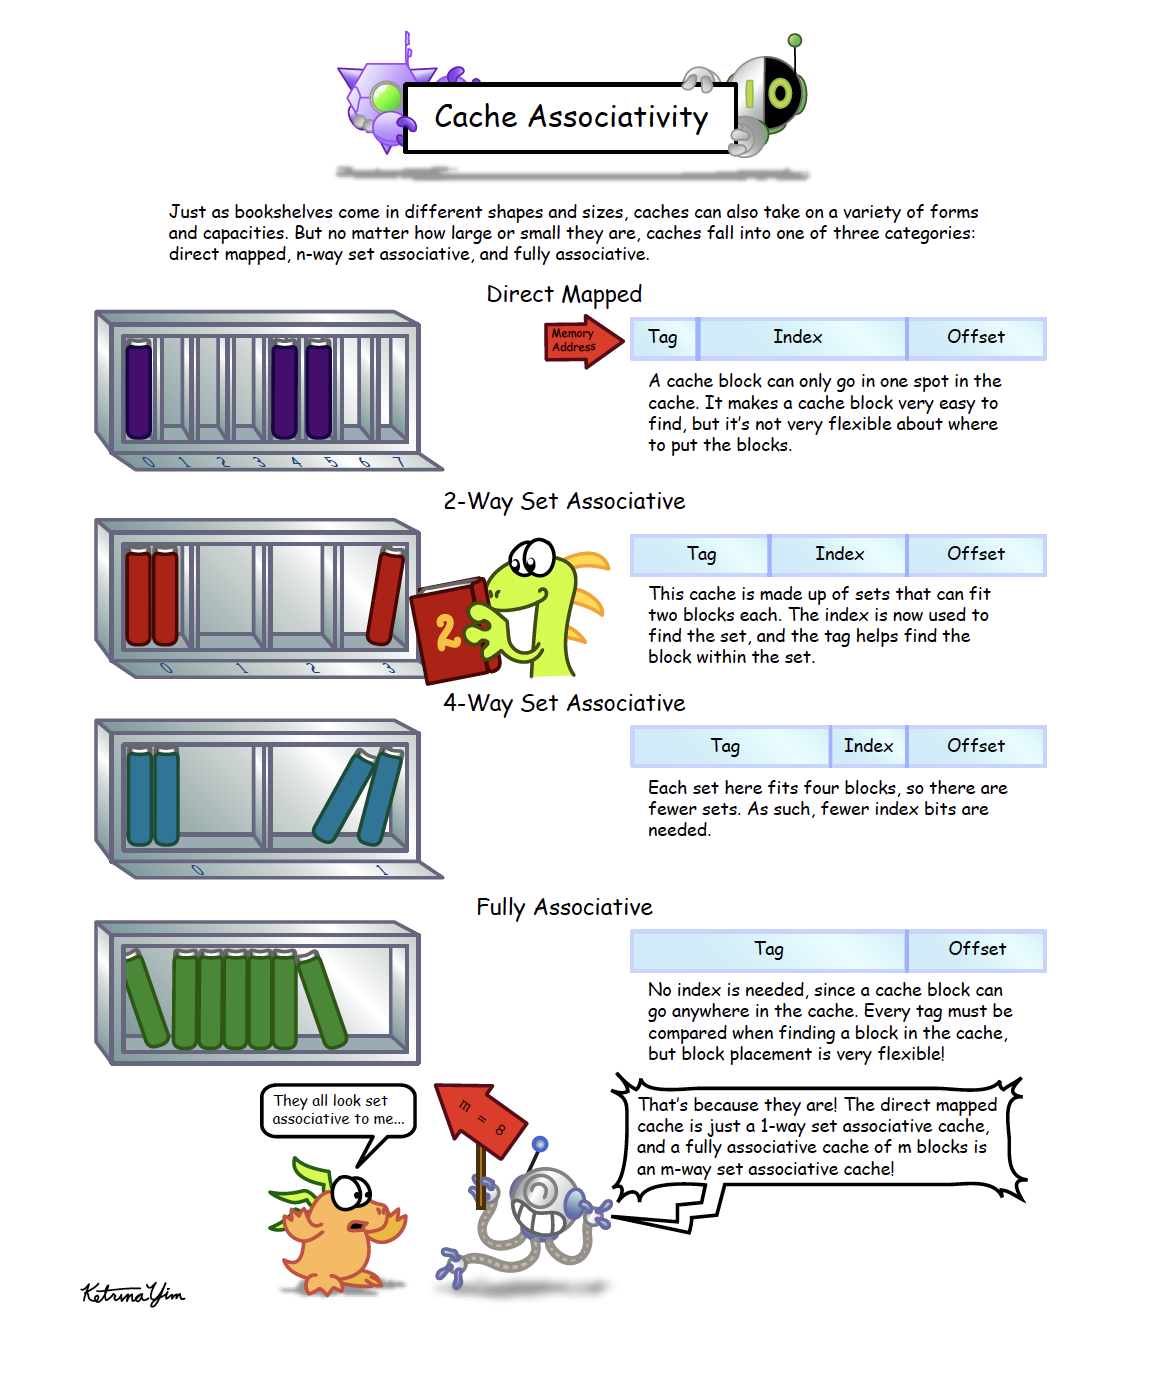
\includegraphics[width=0.7\linewidth]{r1}
		\caption{Interesting Illustration of Set-Associated Cache}
		\label{fig:r1}
	\end{figure}
	\begin{figure}[!h]
		\centering
		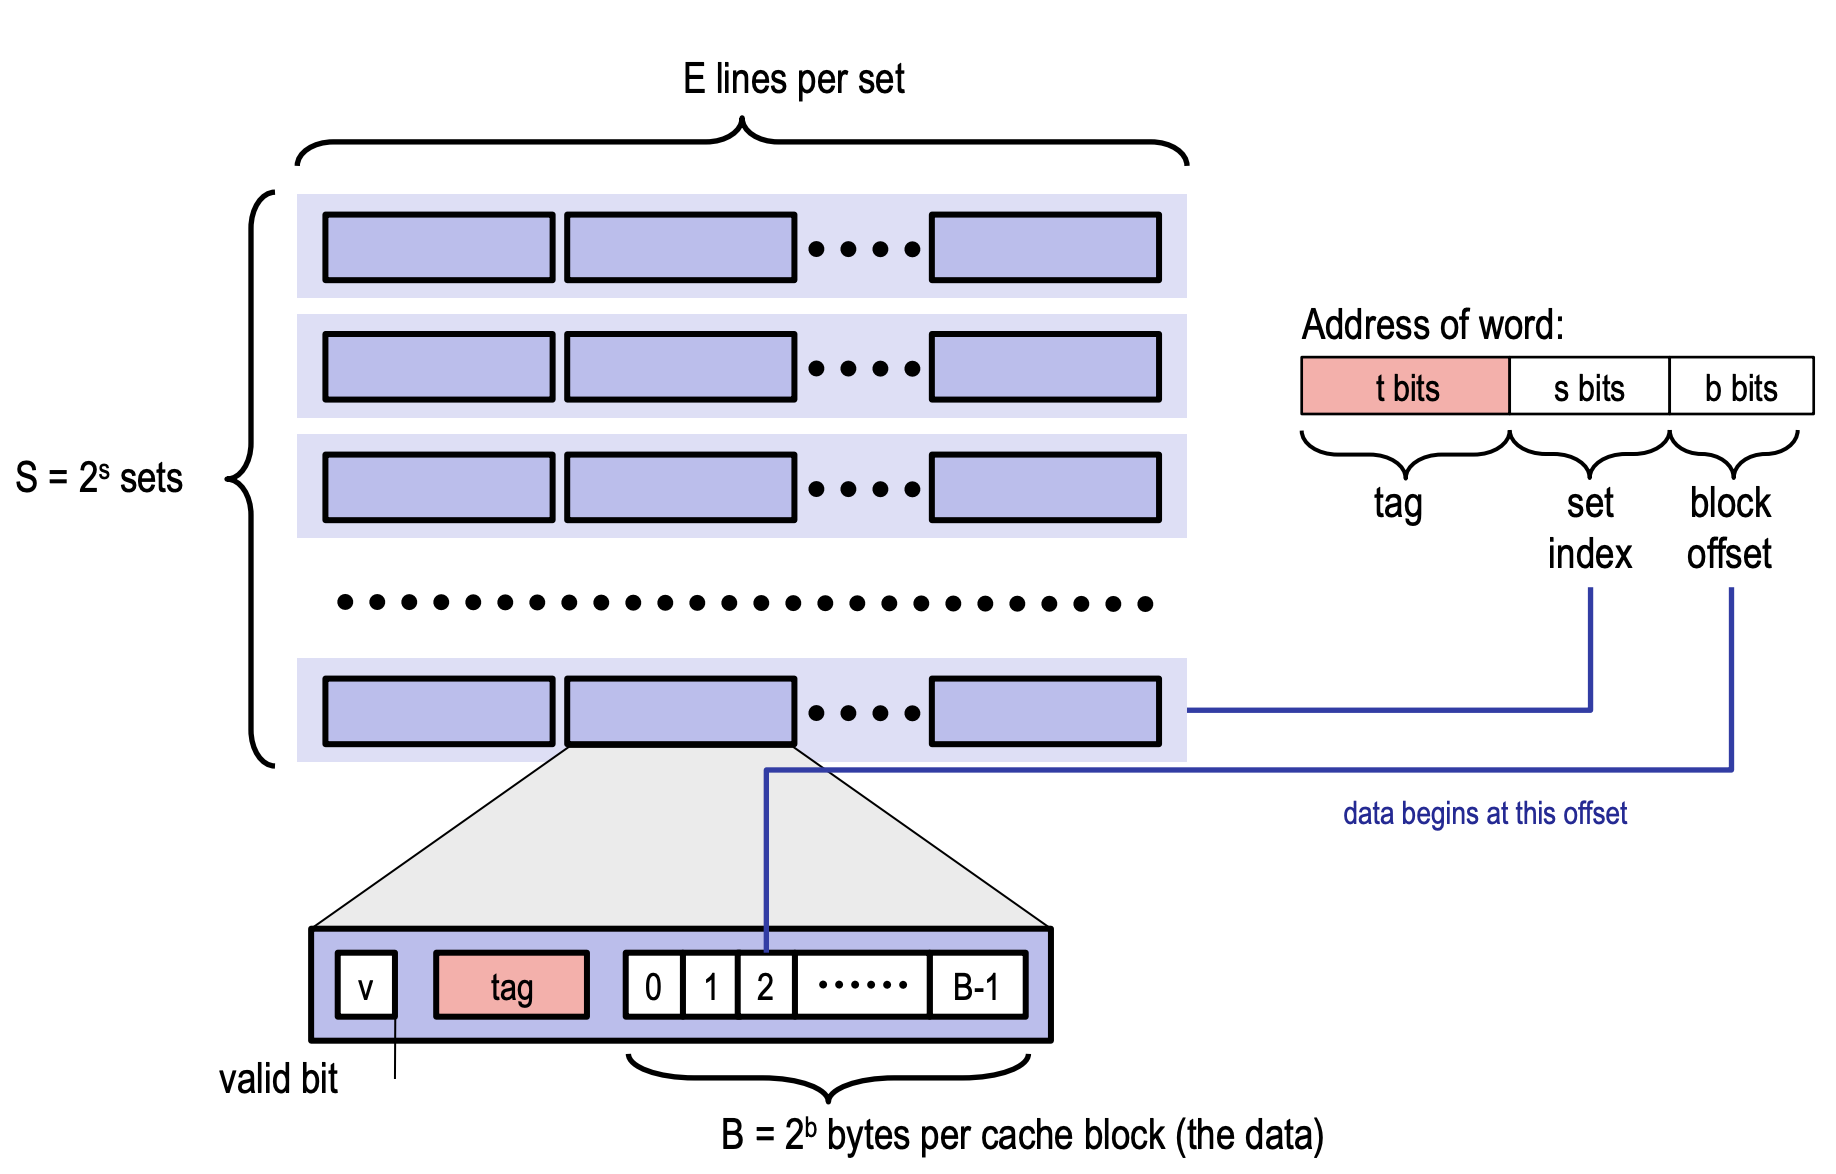
\includegraphics[width=0.7\linewidth]{r2}
		\caption{Abstract of Mapping}
		\label{fig:r2}
	\end{figure}
	

	\item \textbf{Hints}
	
	In this part, the cache is just 2D array of cache lines: 
	\begin{itemize}
		\item \lstinline|struct cache_line cache[S][E]|
		\item 	S=$ 2^s $,is the number of sets
		\item 	E is associativity
	\end{itemize}
	Each cache line has: Valid bit,Tag, LRU counter
	
	\item \textbf{Cache Replacement}
	
	In this lab, we utilize \textbf{LRU} to replace missed cache block. LRU is –	Least	Recently	Used	replacement	policy.  It evicts	the	least	recently	used	block	from	the	cache	to	make	room		for	the	next	block. We could simply use a \textbf{queue} or \textbf{Time Stamps} to implement this. Alg.\ref{algo_disjdecomp} shows the basic idea of LRU used in this lab.~\cite{bryant2003computer}
	\begin{algorithm} \SetKwData{Left}{left}\SetKwData{This}{this}\SetKwData{Up}{up} \SetKwFunction{Union}{Union}\SetKwFunction{FindCompress}{FindCompress} \SetKwInOut{Input}{input}\SetKwInOut{Output}{output}
		
		\Input{Blocks Set $ B = \{ b_1, b_2, ... , b_n\} $} 
		\Output{Replaced Block $ b $}
		\BlankLine 
		
		Define $ t_{min} = \infty $\\
		Define $ ir = 0$ \\
		\For{$ each\ b_i\ in\ B  $}{ 
				\If()
				{$ b_i.t \leq t_{min} $}{\label{lt} 
					$ t_{min}=b_{i}.t; $\\
					$ ir=i; $
			}
		}
	\Return $ b_ir $ 
		\caption{LRU Replacement}
		\label{algo_disjdecomp} 
	\end{algorithm}

\item \textbf{Parse \textit{valgrind} File}

Generated by \textit{valgrind}, a open source memory leaking detective tools will play a role in inserting files as the input of \lstinline|csim.c|. To sparse the UNIX command line and file manupulations, pleases refer to \lstinline|getopy()| and \lstinline|fscanf()| in assignment. I'm gonna disscuss the \lstinline|trace| file, which is used to test our cache and compared to \lstinline|csim_ref|. Generally, there're 4 operations here in \lstinline|trace|.
\begin{itemize}
	\item \textbf{I}. \underline{Instruction Load}. Just ignore it in our lab because we only focus on data load/store.
	\item \textbf{L}. \underline{Data Load}. It may cause: 1) hit (data in cache) 2) miss (data not in cache) 3) miss eviction (conflicts occur when load data from main memory to cache)
	\item \textbf{S}. \underline{Data Store}. It may cause: 1) hit (data in cache) 2) miss (data not in cache) 3) miss eviction (conflicts occur when load data from main memory to cache). Exactly same as \textbf{L}
	\item \textbf{M}. \underline{Data Modify}. It may cause: 1) 2 hits (data in cache) 2) miss + hit  (data not in cache) 3) miss eviction + hit (conflicts occur when load data from main memory to cache). \textbf{M} is just a \textbf{S} after \textbf{L}. Pls kindly understand this because it's very vital next.
\end{itemize}

\end{itemize}




\subsubsection{Code}

I'm gonna attach some \underline{core} code only in this section, for details, please refer to my source code uploaded.

First of all, I defined a \textbf{basic data structure} for cache line. 
\begin{lstlisting}[language=c]
// primary data structure
typedef struct {
	int valid;  // valid bit, 0 is invalid, 1 is valid
	int tag;    // tag bit
	int time;   // LRU time, manupulate LRU
} cache_line;
// abstract of cache
//*   *cache specifies each sets, **cache specifies each block   *//
cache_line** cache;
\end{lstlisting}

Remember that \lstinline|S| for sets, \lstinline|E| for ways, \lstinline|b| for blocks. To manupulate each cache block, I defined \lstinline|index_s|,  \lstinline|index_E|,  \lstinline|index_b|. They're all set to the \textbf{global variebles}. Take a look at the following code:
\begin{lstlisting}[language=c]
// parameters definition
int S;                 // num of sets
int E;                 // num of ways == lines per set
int B;                 // block size
int index_s;           // store the index of sets when allocates
int index_E;           // store the index of lines in a set.
int index_b;           // store the index of blocks in memory
int current_time;      // manupulate LRU replacement
char input_file[100];  // input file generated by others
FILE* file_pointer;    // manupulate input_file
\end{lstlisting}

The \lstinline|main| function of the code is divided into 3 main parts:
\begin{enumerate}
\item parse the command
\item preparation work, including legal check, global variable initialization
\item function call including \lstinline|init_cache()|, \lstinline|operation_parse()|, \lstinline|free_cache()|, \lstinline|fclose(file_pointer)|, \lstinline|printSummary(hits, misses, evictions)|. We'll talk about them later.
\end{enumerate}

For the \textbf{parse command section}, referred to materials from CMU, it mainly works with \lstinline|getopt()| as follows:
\begin{lstlisting}[language=c]
// parse command line
while ((params = getopt(argc, argv, "s:E:b:t:hv")) != -1) {
	switch (params) {
		// just list a few, the complete version refers to the source code pls
		case 's':
		index_s = atoi(optarg);
		break;
		case 'E':
		index_E = atoi(optarg);
		break;
		case 'b':
		index_b = atoi(optarg);
		break;
	}
}
\end{lstlisting}

For \textbf{preparation work}, we're gonna check if all \lstinline|index| is correct(at least $\geq$ 0 ) and examines whether files in \lstinline|./trace| are work. \lstinline|S|, \lstinline|B|, \lstinline|E| could be derived from 64-bit address in this lab, just by \lstinline|<<| is enough. That's why we utilize power of 2 for convenience. 

For \textbf{function calls}, here're the APIs I'm gonna use later:
\begin{lstlisting}[language=c]
// let's begin
init_cache();                           // initialize cache
operation_parse();                      // parse instructions in input file
free_cache();                           // free cache real memory
fclose(file_pointer);                   // free file memory
printSummary(hits, misses, evictions);  // report result
\end{lstlisting}

\begin{itemize}
	\item \lstinline|init_cache()|:
	
	We will use \lstinline|malloc| to allocate memory for a specific cache object. Due to 2-level pointer I used here for cache, cache itself has a capacity of \lstinline|S| and each cache[i] has a capacity of \lstinline|E| in general. We initialize all of them with \lstinline|valid = 0|, \lstinline|-1| for \lstinline|tag| and \lstinline|time|.
	\begin{lstlisting}[language=c]
void init_cache() {
	// malloc for a new cache
	//* for a cache at the top, it has a memory size of S
	cache = (cache_line**)malloc(sizeof(cache_line*) * S);
	// clear all zeros
	for (int i = 0; i < S; ++i) {
		//* for each set, it has a memory size of E
		cache[i] = (cache_line*)malloc(sizeof(cache_line) * E);
		for (int j = 0; j < E; ++j) {
			cache[i][j].valid = 0;
			cache[i][j].tag = -1;
			cache[i][j].time = -1;
		}
	}
}
	\end{lstlisting}

\item \lstinline|operation_parse()|

From the \lstinline|./trace| file, we need to use \lstinline|fscanf| (recommended by assignment) to sparse the instruction. \textbf{I, L, S, M} are the 4 cases we care about. It could usually be implemented by a \lstinline|switch| to sparse. For \textbf{I}, as mentioned before, we just \lstinline|continue| it. And for \textbf{L} or \textbf{S}, we call \lstinline|update_cache(address)| to do place and replace. Note that for \textbf{M}, as we treated it as \textbf{S}after \textbf{L} we should maintain the order of each case in the \lstinline|switch|, which means no \lstinline|break| should be there to correct its executing order.~\cite{lecture}
\begin{lstlisting}[language=c]
void operation_parse() {
	unsigned int address;  // address, 2nd argument
	int size;  // size, the number of bytes accessed by the operation, 3rd
	// argument
	char operation;
	char command;  // manupulate, -v, -t, -h
	
	while (fscanf(file_pointer, "%c %xu%c%xu ", &operation, &address, &command,
	&size) > 0) {
		switch (operation) {
			case 'I':  // I: just continue
			continue;
			case 'L':  // L
			update_cache(address);
			break;
			case 'M':  // M
			update_cache(address);
			case 'S':  // S
			update_cache(address);
			break;
			default:
			break;
		}
		update_time(); // plus each cache line's time 1 in every visit
	}
}
\end{lstlisting}

\item \lstinline|free_cache()|

It's a simple loop for a 2-level pointer to free memory allocation

\item \lstinline|update_cache(unsigned int address)|

{\color{red} This is the most vital part in partA}. The logic is simple, which is 
\begin{enumerate}
	\item Parse the instruction we got before to make it clear about which is exactly the corresponding set number of tag value. Set number will be stored in \lstinline|set_spec|, tag value will be stored in \lstinline|tag_spec|. As the 64-bit address is conducted as \lstinline|tag set offset |, I used a \lstinline|AND| and right shift operation to get that.
	\item search in the cache set by comparing \lstinline|tag| and check \lstinline|valid|
	\subitem If hit, update and return.
	\subitem If not hit, go to next step.
	\item Search in the set for the empty space to replace.
	\subitem If found, update and return.
	\subitem If not found, go to next step
	\item Use \textbf{LRU} to replace the block. Update and return. The \textbf{LRU} is implemented by a \textbf{time stamp}, algorithm logic is shown before in Alg.\ref{algo_disjdecomp}
\end{enumerate}
	\begin{lstlisting}[language=c]
void update_cache(unsigned int address) {
	// sparse tag value
	// address: |tag|set|offset|
	int tag_spec =
	(address >> (index_b + index_s));  // address right shift for
	// index_b+index_s sparse set value
	int set_spec =
	(address >> index_b) &
	((0xFFFFFFFF) >> (64 - index_s));  // it should be |set|, bit-wise AND
	// could sparse |set| from origin
	// look up in a set
	for (int i = 0; i < E; ++i) {
		/* hit: tag is matched && valid == 1 */
		if ((cache[set_spec][i].tag == tag_spec) && cache[set_spec][i].valid == 1) {
			hits++;  // hit plus 1
			cache[set_spec][i].time =
			current_time;  // update the visit time to do LRU
			return;
		}
	}
	for (int i = 0; i < E; ++i) {
		// invalid --- miss
		if (cache[set_spec][i].valid == 0) {
			cache[set_spec][i].valid = 1;  // turn to valid
			cache[set_spec][i].tag = tag_spec;
			cache[set_spec][i].time = current_time;
			misses++;
			return;
		}
	}
	// valid but not match --- eviction
	evictions++;
	misses++;
	//******* LRU replacement *******//
	int min_time = 10000;  // simulate \infty
	int ir;                // replaced block
	for (int i = 0; i < E; ++i) {
		if (cache[set_spec][i].time < min_time) {
			min_time = cache[set_spec][i].time;  // update time
			ir = i;                              // update ir
			/* code */
		}
	}
	// after LRU, ir is what we're gonna replace
	cache[set_spec][ir].tag = tag_spec;
	cache[set_spec][ir].time = current_time;
}
	\end{lstlisting}
\item \lstinline|update_time()| is just doing plus 1 each time
\end{itemize}

\lstinline|man_help()|, \lstinline|-h|, \lstinline|-v| and \lstinline|-t| is ignored here. They're not important and used for debugging and using exclusively. 

\subsubsection{Evaluation}

\lstinline|>>make clean| and \lstinline|make| in the directory, then \lstinline|./python.py| by Python2.x interpreter. The result is shown as Fig.\ref{fig:1} and \textbf{reached full mark of 27}.
\begin{figure}[!h]
	\centering
	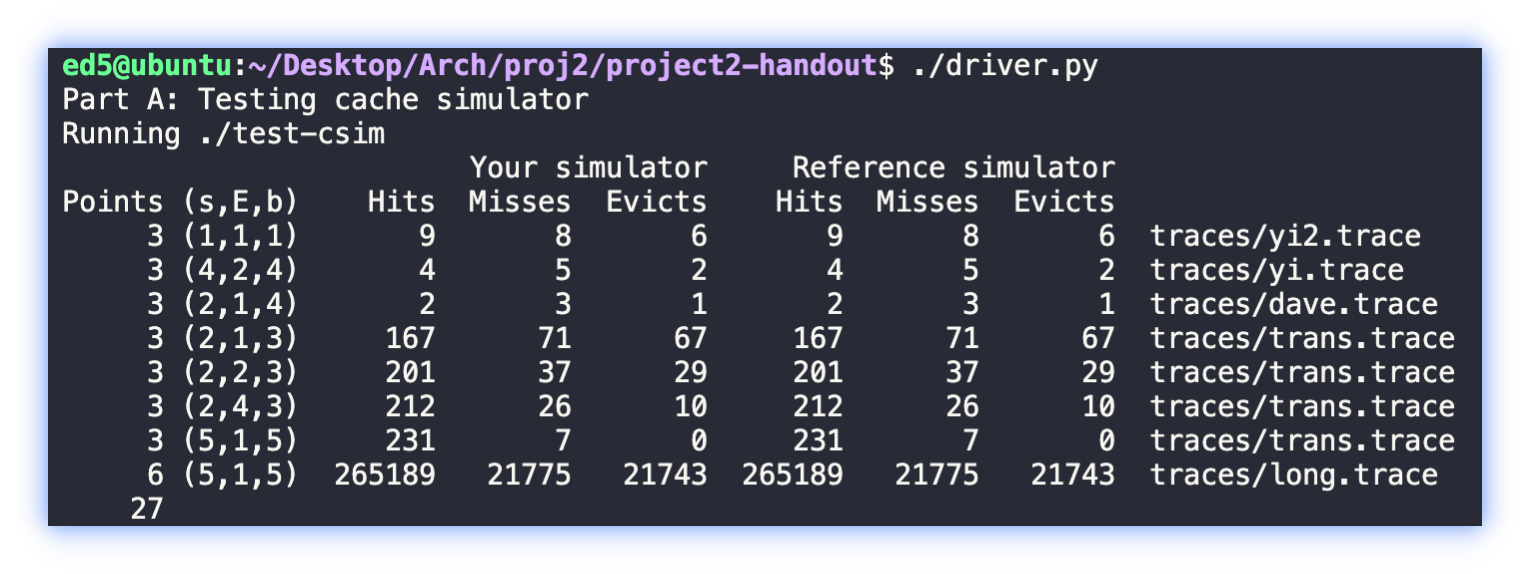
\includegraphics[width=\linewidth]{1}
	\caption{test in PartA}
	\label{fig:1}
\end{figure}

\subsection{Part B}

\subsubsection{Techniques}

In this part, we're gonna implement an optimized \lstinline|transpose_submit(int M, int N, int A[N][M], int B[M][N])| in \lstinline|trans.c| to transpose a fixed size matrix. The reasons why we need to deal with it is \textbf{principles of locality}, both \textbf{tempory} and \textbf{spatial}. As a matrix is \textbf{2-dimension} in this lab and the store strategy of it is \textbf{row-first}, we need to use specific tricks to reduce misses. The main technique here is we called, \textbf{Blocking}. 

\textbf{Blocking} can significantly improve the temporal locality of inner loops. The
general idea of blocking is to organize the data structures in a program into large chunks called \textit{blocks}. To implement this we usually introduces \textbf{stride} which is very common in \textbf{machine learing} or \textbf{parallelisim computing} research fields. In fact, a very popular simulator, \lstinline|zSim|~\cite{sanchez2013zsim} proposes by MIT and Stanford back to 2013 has utilized some of the ideas to reality. 

\begin{figure}[!h]
	\centering
	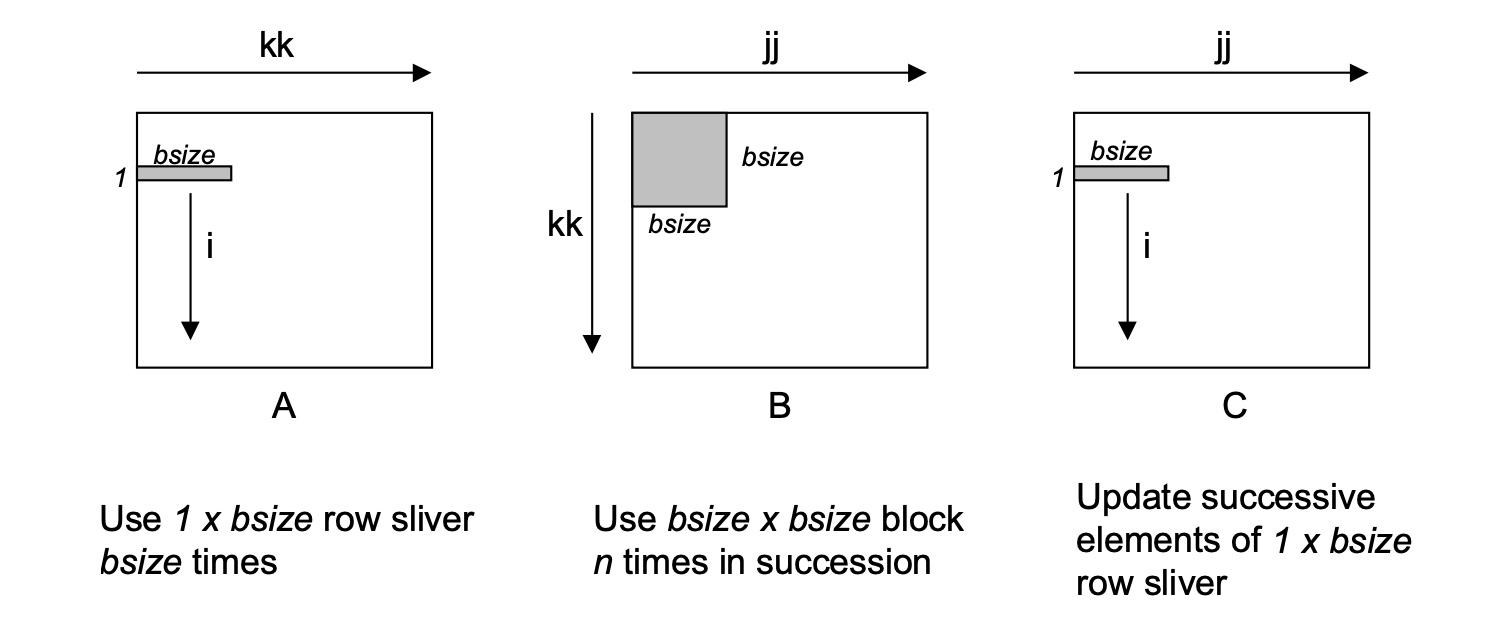
\includegraphics[width=0.8\linewidth]{r3}
	\caption{\textbf{Graphical interpretation of blocked matrix multiply}: The innermost $ (j, k) $ loop pair multiplies a $ 1 \times $ $ bsize $ sliver of \lstinline|A| by a $ bsize \times bsize $ block of \lstinline|B| and accumulates into a $ 1 \times bsize $ sliver of \lstinline|C|}
	\label{fig:r3}
\end{figure}

The classic example of this is \textbf{matrix multiplication} shown in Fig.\ref{fig:r3}. We also utilized blocking in \textbf{matrix transpose}. They're quite similar.

\subsubsection{Analysis}

In this part, we're gonna use cache placement strategies of \textbf{$ s $=5, $ E $=1, $ b $=5}, which means that there're totally $ 2^5 = 32 $ sets, and using direct-mapping ($ E=1 $) way. Block size is $ 2^5=32 $ (contains $ 8 $ \lstinline|int|)too. So, for a single cache set, we could store $ 8 $ \lstinline|int| at a time. For a single cache, we could store $ 32 \times 8 $ \lstinline|int| at a time. 

The testbench is buit on three different sizes of matrixes: $ 32 \times 32 $, $ 64 \times 64 $, $ 61 \times 67 $. We'll seperately optimize them.

\subsubsection{Code}

{\color{blue} $ 32 \times 32 $}

A cache line could contain \textbf{8} \lstinline|int|, in the original $ 32 \times 32 $ matrix, we have \textbf{32} integers per row, which can be contained by \textbf{4} cache line. A cache could contain \textbf{8} rows, so we divide the $ 32 \times 32 $ matrix into \textbf{8} $\times$ \textbf{8} block chunks. In a inner-chunk, we did transposition. (line $\rightarrow$ column).

Note that if the data is on the main diagonal, we won't tanspose immediately. If so, we could reduce the 2 misses happened when transpositon at diagonal. I declared \lstinline|tmp| to store the value and \lstinline|index| to store its position. After the other data has been transposed, we could directly assign the \textbf{8} diagonal value at a time. The code is:
\begin{lstlisting}[language=c]
int i, j, tmp, index;
int row_Block, col_Block;  // top row and column manupulation with stride
	
if (M == 32) {  // divide the the 32X32 block into 8X8 , decrease the number
	// of misses
	// stride is 8, for 8X4=32, each 
	for (row_Block = 0; row_Block < N; row_Block += 8) {
		for (col_Block = 0; col_Block < M; col_Block += 8) {
			for (i = row_Block; i < row_Block + 8; i++) {
				for (j = col_Block; j < col_Block + 8; j++) {
					if (i != j) {
						B[j][i] = A[i][j]; // tanspose 
					} else {
						tmp = A[i][j];  // i==j means the data is on the diagonal. if we
						// set B right now ,the  misses and
						// evictions will increase . because
						// the cache set of B is same to A.
						index = i;}}
				if (col_Block == row_Block) {  // just set B on the diagonal. other
					// than shouldn't set the B
					B[index][index] = tmp; }}}}}
\end{lstlisting}

The theorical optimal result is \textbf{256} misses. To save pages, I'm not gonna talk about why it is. Maybe I'll work on that by coding in the future.

{\color{blue} $ 64 \times 64 $}

The part is much more difficult than the other 2, basically, we're gonna divide it into 64 \textbf{8} $\times$ \textbf{8} blocks. But here're some tricks. 

The first trick is we call \textbf{Read All Only Once} that shows from code line10 $\rightarrow$ 17. To be more specific, when doing blocking, {we read the \underline{fullline of the block} once}. For example, the matrix $ A $ has the size 32 $\times$ 32. When CPU reads $ A[0][0] $, one cache line is filled with $ A[0][0],A[0][1], ...,A[0][7] $ because row-first. If we just read one element like $ A[0][6] $ then transpose the element and get the value of $ B[6][0] $, the cache line is replaced with $ B[0][0], ...,B[0][7]. $Thus, there are extra elements that are not read but placed in the cache. If we not use them in this time, they are still in requirement. We can read these elements at one time.

The second trick we call is \textbf{Save and Load}. ~\cite{zhihu}. To be specific, in 64 $\times$ 64 matrix, the cache can store \textbf{4} rows of matrix. But if we perform \textit{blocking} of 8 $\times$ 8, it can only be filled with \textit{line1} to \textit{line4} or \textit{line5} to \textit{line8}. What we're gonna do is dividing it into \textbf{more fine-grained}. As mentioned before, we first read 4 elements in A's lower left quarter and store the transposition of them in B's lower left quarter.This is called \textit{Save}. Then,when transposing A's upper right corner, we first \textit{load} the elements in B we store before and do the transposition of the upper right corner and the lower left corner of B. 

\begin{lstlisting}[language=c]
	// using 4 + 8 = 12 variable, following coding style
	int t, t1, t2, t3, t4, t5, t6, t7, t8;
	for (row_Block = 0; row_Block < N; row_Block += 8)
	for (col_Block = 0; col_Block < M; col_Block += 8)  // 8X8 blocking
	{  // inner is blocking 4X4
		// save and load
		for (t = row_Block; t < row_Block + 4; ++t) {
			// read all only once
			t1 = A[t][col_Block];
			t2 = A[t][col_Block + 1];
			t3 = A[t][col_Block + 2];
			t4 = A[t][col_Block + 3];
			t5 = A[t][col_Block + 4];
			t6 = A[t][col_Block + 5];
			t7 = A[t][col_Block + 6];
			t8 = A[t][col_Block + 7];
			
			B[col_Block][t] = t1;
			B[col_Block + 1][t] = t2;
			B[col_Block + 2][t] = t3;
			B[col_Block + 3][t] = t4;
			B[col_Block][t + 4] = t5;
			B[col_Block + 1][t + 4] = t6;
			B[col_Block + 2][t + 4] = t7;
			B[col_Block + 3][t + 4] = t8;
		}
		for (t = col_Block; t < col_Block + 4; ++t) {
			t1 = A[row_Block + 4][t];
			t2 = A[row_Block + 5][t];
			t3 = A[row_Block + 6][t];
			t4 = A[row_Block + 7][t];
			t5 = B[t][row_Block + 4];
			t6 = B[t][row_Block + 5];
			t7 = B[t][row_Block + 6];
			t8 = B[t][row_Block + 7];
			
			B[t][row_Block + 4] = t1;
			B[t][row_Block + 5] = t2;
			B[t][row_Block + 6] = t3;
			B[t][row_Block + 7] = t4;
			B[t + 4][row_Block] = t5;
			B[t + 4][row_Block + 1] = t6;
			B[t + 4][row_Block + 2] = t7;
			B[t + 4][row_Block + 3] = t8;
		}
		for (t = row_Block + 4; t < row_Block + 8; ++t) {
			t1 = A[t][col_Block + 4];
			t2 = A[t][col_Block + 5];
			t3 = A[t][col_Block + 6];
			t4 = A[t][col_Block + 7];
			B[col_Block + 4][t] = t1;
			B[col_Block + 5][t] = t2;
			B[col_Block + 6][t] = t3;
			B[col_Block + 7][t] = t4; }}
\end{lstlisting}

The theorical optimal result is \textbf{1024} misses. 

{\color{blue} $ 61 \times 67 $}

Totally like {\color{blue} $ 32 \times 32 $}, we made a chunk of block, \textbf{16}$ \times $\textbf{16}, and here's the code:
\begin{lstlisting}[language=c]
// separate the the 61X67 block into 16X16 , decrease the number of misses
for (row_Block = 0; row_Block < N; row_Block += 16) {
	for (col_Block = 0; col_Block < M; col_Block += 16) {
		for (i = row_Block; i < row_Block + 16 && (i < N); i++) {
			for (j = col_Block; j < col_Block + 16 && (j < M); j++) {
				if (i != j) {
					B[j][i] = A[i][j];
				} else {
					tmp = A[i][j];  // i==j means is the diagonal. if we
					// set B right now ,the  misses and
					// evictions will increase . because
					// the cache set of B is same to A.
					index = i; }}
			if (col_Block == row_Block) {  // just set B on the diagonal. other
				// than shouldn't set the B
				B[index][index] = tmp; }}}}
\end{lstlisting}

\subsubsection{Evaluation}

{\color{blue} \lstinline|./test-trans -M 32 -N 32|}
\begin{table}[!h]
	\centering  % 显示位置为中间
	\label{table1}  % 用于索引表格的标签
	\begin{tabular}{| m{3cm} | m{3cm} | m{3cm} |}
		\hline  % 表格的横线
		hits&misses&evictions \\  % 表格中的内容,用&分开,\\表示下一行
		\hline
		1766&\textbf{287}&255 \\
		\hline
	\end{tabular}
\end{table}


{\color{blue} \lstinline|./test-trans -M 64 -N 64|}
\begin{table}[!h]
	\centering  % 显示位置为中间
	\label{table1}  % 用于索引表格的标签
	\begin{tabular}{| m{3cm} | m{3cm} | m{3cm} |}
		\hline  % 表格的横线
		hits&misses&evictions \\  % 表格中的内容,用&分开,\\表示下一行
		\hline
		9066&\textbf{1179}&1147 \\
		\hline
	\end{tabular}
\end{table}

{\color{blue} \lstinline|./test-trans -M 61 -N 67|}
\begin{table}[!h]
	\centering  % 显示位置为中间
	\label{table1}  % 用于索引表格的标签
	\begin{tabular}{| m{3cm} | m{3cm} | m{3cm} |}
		\hline  % 表格的横线
		hits&misses&evictions \\  % 表格中的内容,用&分开,\\表示下一行
		\hline
		6197&\textbf{1985}&1953 \\
		\hline
	\end{tabular}
\end{table}


By {\color{blue} \textit{linux} $>>$ \lstinline|./driver.py|}, we could get the complete evaluation result at a time.The result is shown in Fig.\ref{fig:2} and luckily I \textbf{reached full mark of 26. }

\textbf{Combined patA and partB, I got the full mark of 53!}
\begin{figure}[!h]
	\centering
	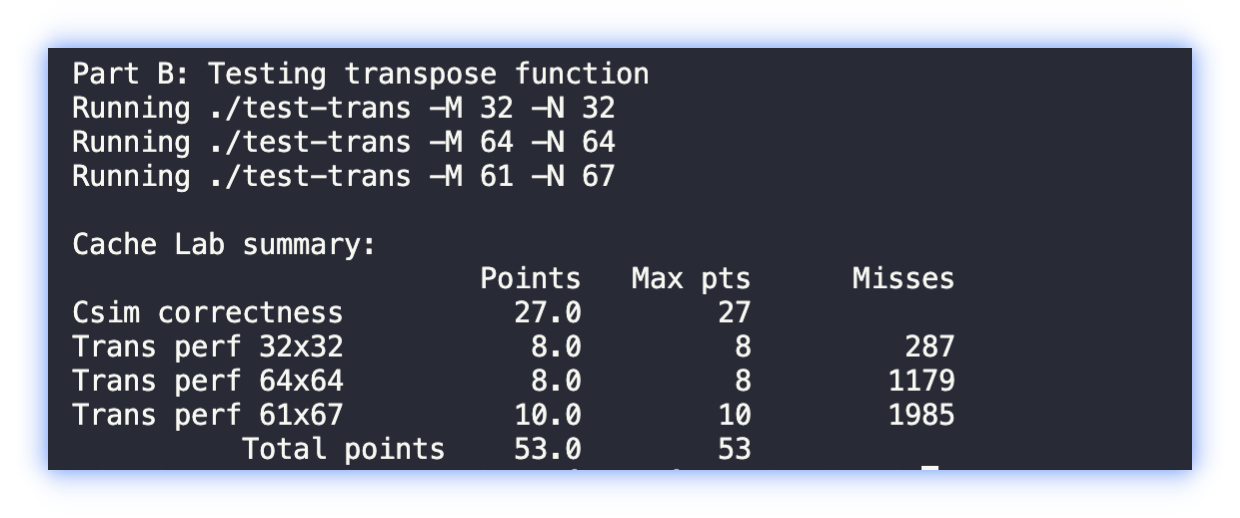
\includegraphics[width=\linewidth]{2}
	\caption{test for PartB}
	\label{fig:2}
\end{figure}


\section{Conclusion}

\subsection{Problems}
\begin{enumerate}
	\item In Part A, building the structure of the simulator from zero is quite hard to understand. It takes some effort to further understand and make it clear what we should do by dividing the stages into \textbf{1) placement 2)replacement. }
	\item In Part B, it's hard to make it clear how the \textit{\textbf{Blocking}} works because code with \textit{blocking} is difficult to wirte and read. However, I scanned materials from CMU and got to know how to optimize the function.
	\item It's hard to get the full score when constructing 64 $\times$ 64 matrix compared to the others. I've read many articles and looked deep into the theory behind behaviors with endless efforts and tries. And it works.
	\item It's a little bit hard to understand how SOTA of performing, but it is actually very interesting.
\end{enumerate}

\subsection{Achievements}

\begin{itemize}
	\item Successfully build a cache simulation \lstinline|csim.c|, with the same output as \lstinline|csim-ref|. 
	\item Use \textit{Blocking} with 2 other tricks in the guidance of principles of locality to optimize 3 differrent matrix sizes tests. 
	\item Construct a number of testbenches to compare different techniques.
	\item Write all the codes with verbose comments. Follow the coding style correctly. Make it readable and easy to understand.
	\item Write code and instruction basiclally on what we're truly understand and try to build a software and hardware co-design method to implement taht kind of stuff.
\end{itemize}

 



\bibliographystyle{plain}
\bibliography{ref}


%----------------------------------------------------------------------------------------


\end{document}